
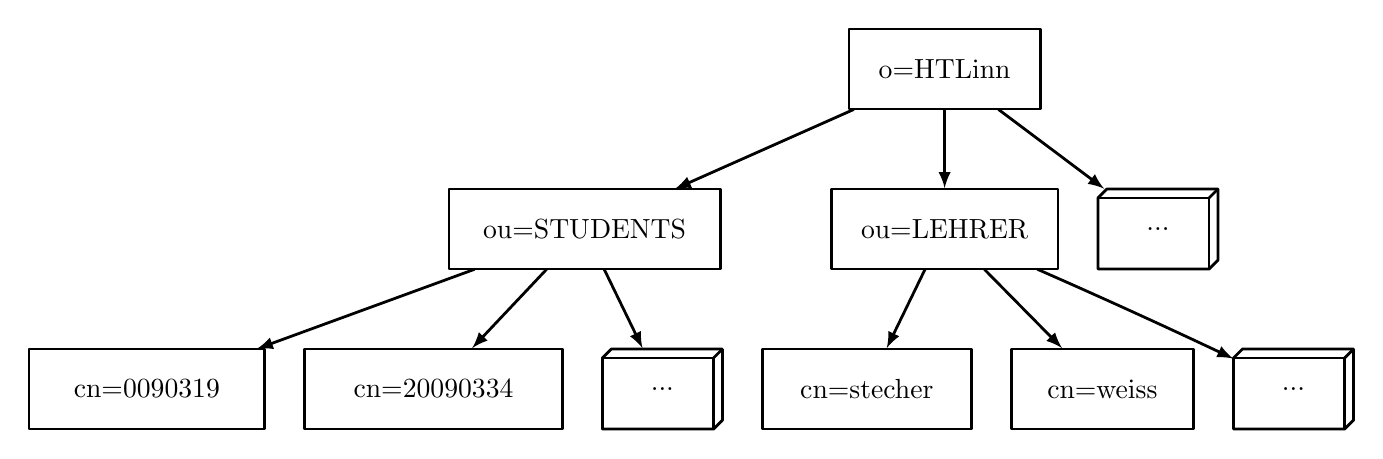
\begin{tikzpicture}[>=latex,line join=bevel,scale=0.8]
  \pgfsetlinewidth{1bp}
%%
\pgfsetcolor{black}
  % Edge: ou=LEHRER -> cn=weiss
  \draw [->] (429.92bp,71.831bp) .. controls (438.34bp,63.285bp) and (448.54bp,52.944bp)  .. (464.84bp,36.413bp);
  % Edge: ou=LEHRER -> cn=stecher
  \draw [->] (403.17bp,71.831bp) .. controls (399.3bp,63.877bp) and (394.68bp,54.369bp)  .. (385.95bp,36.413bp);
  % Edge: ou=STUDENTS -> cn=0090319
  \draw [->] (200.54bp,71.924bp) .. controls (173.73bp,62.124bp) and (140.41bp,49.945bp)  .. (102.48bp,36.083bp);
  % Edge: ou=STUDENTS -> ...  
  \draw [->] (258.83bp,71.831bp) .. controls (262.7bp,63.877bp) and (267.32bp,54.369bp)  .. (276.05bp,36.413bp);
  % Edge: ou=LEHRER -> ... 
  \draw [->] (453.65bp,71.953bp) .. controls (474.97bp,62.59bp) and (501.51bp,50.752bp)  .. (541.94bp,31.691bp);
  % Edge: o=HTLinn -> ou=STUDENTS
  \draw [->] (371.12bp,143.83bp) .. controls (349.45bp,134.2bp) and (322.66bp,122.29bp)  .. (290.59bp,108.04bp);
  % Edge: ou=STUDENTS -> cn=20090334
  \draw [->] (232.84bp,71.831bp) .. controls (224.85bp,63.369bp) and (215.2bp,53.149bp)  .. (199.39bp,36.413bp);
  % Edge: o=HTLinn -> ou=LEHRER
  \draw [->] (412bp,143.83bp) .. controls (412bp,136.13bp) and (412bp,126.97bp)  .. (412bp,108.41bp);
  % Edge: o=HTLinn -> ...
  \draw [->] (436.22bp,143.83bp) .. controls (448.16bp,134.88bp) and (462.73bp,123.96bp)  .. (483.78bp,108.16bp);
  % Node: cn=stecher
\begin{scope}
  \definecolor{strokecol}{rgb}{0.0,0.0,0.0};
  \pgfsetstrokecolor{strokecol}
  \draw (424bp,36bp) -- (330bp,36bp) -- (330bp,0bp) -- (424bp,0bp) -- cycle;
  \draw (377bp,18bp) node {cn=stecher};
\end{scope}
  % Node: ...
\begin{scope}
  \definecolor{strokecol}{rgb}{0.0,0.0,0.0};
  \pgfsetstrokecolor{strokecol}
  \draw (535bp,108bp) -- (485bp,108bp) -- (481bp,104bp) -- (481bp,72bp) -- (531bp,72bp) -- (535bp,76bp) -- cycle;
  \draw (531bp,104bp) -- (481bp,104bp);
  \draw (531bp,104bp) -- (531bp,72bp);
  \draw (531bp,104bp) -- (535bp,108bp);
  \draw (508bp,90bp) node {...};
\end{scope}
  % Node: ... 
\begin{scope}
  \definecolor{strokecol}{rgb}{0.0,0.0,0.0};
  \pgfsetstrokecolor{strokecol}
  \draw (596bp,36bp) -- (546bp,36bp) -- (542bp,32bp) -- (542bp,0bp) -- (592bp,0bp) -- (596bp,4bp) -- cycle;
  \draw (592bp,32bp) -- (542bp,32bp);
  \draw (592bp,32bp) -- (592bp,0bp);
  \draw (592bp,32bp) -- (596bp,36bp);
  \draw (569bp,18bp) node {...};
\end{scope}
  % Node: o=HTLinn
\begin{scope}
  \definecolor{strokecol}{rgb}{0.0,0.0,0.0};
  \pgfsetstrokecolor{strokecol}
  \draw (455bp,180bp) -- (369bp,180bp) -- (369bp,144bp) -- (455bp,144bp) -- cycle;
  \draw (412bp,162bp) node {o=HTLinn};
\end{scope}
  % Node: ou=STUDENTS
\begin{scope}
  \definecolor{strokecol}{rgb}{0.0,0.0,0.0};
  \pgfsetstrokecolor{strokecol}
  \draw (311bp,108bp) -- (189bp,108bp) -- (189bp,72bp) -- (311bp,72bp) -- cycle;
  \draw (250bp,90bp) node {ou=STUDENTS};
\end{scope}
  % Node: ou=LEHRER
\begin{scope}
  \definecolor{strokecol}{rgb}{0.0,0.0,0.0};
  \pgfsetstrokecolor{strokecol}
  \draw (463bp,108bp) -- (361bp,108bp) -- (361bp,72bp) -- (463bp,72bp) -- cycle;
  \draw (412bp,90bp) node {ou=LEHRER};
\end{scope}
  % Node: ...  
\begin{scope}
  \definecolor{strokecol}{rgb}{0.0,0.0,0.0};
  \pgfsetstrokecolor{strokecol}
  \draw (312bp,36bp) -- (262bp,36bp) -- (258bp,32bp) -- (258bp,0bp) -- (308bp,0bp) -- (312bp,4bp) -- cycle;
  \draw (308bp,32bp) -- (258bp,32bp);
  \draw (308bp,32bp) -- (308bp,0bp);
  \draw (308bp,32bp) -- (312bp,36bp);
  \draw (285bp,18bp) node {...};
\end{scope}
  % Node: cn=20090334
\begin{scope}
  \definecolor{strokecol}{rgb}{0.0,0.0,0.0};
  \pgfsetstrokecolor{strokecol}
  \draw (240bp,36bp) -- (124bp,36bp) -- (124bp,0bp) -- (240bp,0bp) -- cycle;
  \draw (182bp,18bp) node {cn=20090334};
\end{scope}
  % Node: cn=weiss
\begin{scope}
  \definecolor{strokecol}{rgb}{0.0,0.0,0.0};
  \pgfsetstrokecolor{strokecol}
  \draw (524bp,36bp) -- (442bp,36bp) -- (442bp,0bp) -- (524bp,0bp) -- cycle;
  \draw (483bp,18bp) node {cn=weiss};
\end{scope}
  % Node: cn=0090319
\begin{scope}
  \definecolor{strokecol}{rgb}{0.0,0.0,0.0};
  \pgfsetstrokecolor{strokecol}
  \draw (106bp,36bp) -- (0bp,36bp) -- (0bp,0bp) -- (106bp,0bp) -- cycle;
  \draw (53bp,18bp) node {cn=0090319};
\end{scope}
%
\end{tikzpicture}

